%%%%%%%%%%%%%%%%%%%%%%%%%%%%%%%%%%%%%%%%%
% a0poster Portrait Poster
% LaTeX Template
% Version 1.0 (22/06/13)
%
% The a0poster class was created by:
% Gerlinde Kettl and Matthias Weiser (tex@kettl.de)
%
% This template has been downloaded from:
% http://www.LaTeXTemplates.com
%
% License:
% CC BY-NC-SA 3.0 (http://creativecommons.org/licenses/by-nc-sa/3.0/)
%
%%%%%%%%%%%%%%%%%%%%%%%%%%%%%%%%%%%%%%%%%

%----------------------------------------------------------------------------------------
%	PACKAGES AND OTHER DOCUMENT CONFIGURATIONS
%----------------------------------------------------------------------------------------

\documentclass[a0,portrait,20pt]{a0poster}

\usepackage{multicol} % This is so we can have multiple columns of text side-by-side
\columnsep=100pt % This is the amount of white space between the columns in the poster
\columnseprule=3pt % This is the thickness of the black line between the columns in the poster

\usepackage[svgnames]{xcolor} % Specify colors by their 'svgnames', for a full list of all colors available see here: http://www.latextemplates.com/svgnames-colors

\usepackage{times} % Use the times font
%\usepackage{palatino} % Uncomment to use the Palatino font

\usepackage{graphicx} % Required for including images
\graphicspath{{figures/}} % Location of the graphics files
\usepackage{booktabs} % Top and bottom rules for table
\usepackage[font=small,labelfont=bf]{caption} % Required for specifying captions to tables and figures

\DeclareCaptionFont{myblue}{\color{RoyalBlue}}
\captionsetup{labelfont={myblue,bf}}

\usepackage{amsfonts, amsmath, amsthm, amssymb} % For math fonts, symbols and environments
\usepackage{wrapfig} % Allows wrapping text around tables and figures
\usepackage[position=top]{subfig}
\graphicspath{{figures/}{../paper/figures/}{./}}
\usepackage{tikz,pgf}
\usetikzlibrary{arrows,positioning}

% \usepackage[doi=false,
%             isbn=false,
%             url=false,
%             bibstyle=authoryear,
%             backend=biber,
%             style=authoryear]{biblatex} %, backend=bibtex
% \AtEveryCitekey{%\clearfield{title}
%     \scriptsize
%     \clearfield{note}
%     \clearfield{pages}
%     \clearfield{volume}%
%     \clearfield{number}
%     \clearlist{location}
%     \clearlist{publisher}
%     \clearname{editor}}
% \renewcommand*{\multicitedelim}{\\}
% \def\bibfont{\Large}
% \renewcommand*{\bibfont}{\huge}
%
% \addbibresource{bib.bib}

\begin{document}

%----------------------------------------------------------------------------------------
%	POSTER HEADER
%----------------------------------------------------------------------------------------

% The header is divided into two boxes:
% The first is 75% wide and houses the title, subtitle, names, university/organization and contact information
% The second is 25% wide and houses a logo for your university/organization or a photo of you
% The widths of these boxes can be easily edited to accommodate your content as you see fit


\begin{minipage}[b]{0.75\linewidth}
\veryHuge \color{NavyBlue} \textbf{Bandwidth extension of musical audio signals with no side information using dilated convolutional neural networks} \color{Black}\\ % Title
\Huge\textit{}\\[2cm] % Subtitle
\huge \textbf{Mathieu Lagrange, F\'elix Gontier}\\[0.5cm] % Author(s)
\huge LS2N, CNRS, \'Ecole Centrale Nantes\\[0.4cm] % University/organization
\end{minipage}
%
\begin{minipage}[b]{0.25\linewidth}

\includegraphics[width=14cm]{figures/logoLs2n.jpg}\\
\end{minipage}

\vspace{1cm} % A bit of extra whitespace between the header and poster content

%----------------------------------------------------------------------------------------

\begin{multicols}{2} % This is how many columns your poster will be broken into, a portrait poster is generally split into 2 columns

%----------------------------------------------------------------------------------------
%	ABSTRACT
%----------------------------------------------------------------------------------------

\color{Navy} % Navy color for the abstract

\begin{abstract}

Bandwidth extension has a long history in audio processing. While speech processing tools do not rely on side information, production-ready bandwidth extension tools of general audio signals rely on side information that has to be transmitted alongside the bitstream of the low frequency part, mostly because polyphonic music has a more complex and less predictable spectral structure than speech.

This paper studies the benefit of considering \textbf{a dilated fully convolutional neural network} to perform the bandwidth extension of musical audio signals \textbf{with no side information} on the \textbf{magnitude spectra}. Experimental evaluation using two public datasets, \textit{medley-solos-db} and \textit{gtzan}, respectively of monophonic and polyphonic music demonstrate that the proposed architecture achieves state of the art performance.

\end{abstract}

%----------------------------------------------------------------------------------------
%	INTRODUCTION
%----------------------------------------------------------------------------------------

\color{SaddleBrown} % SaddleBrown color for the introduction

\section*{Background}

\begin{center}\vspace{1cm}
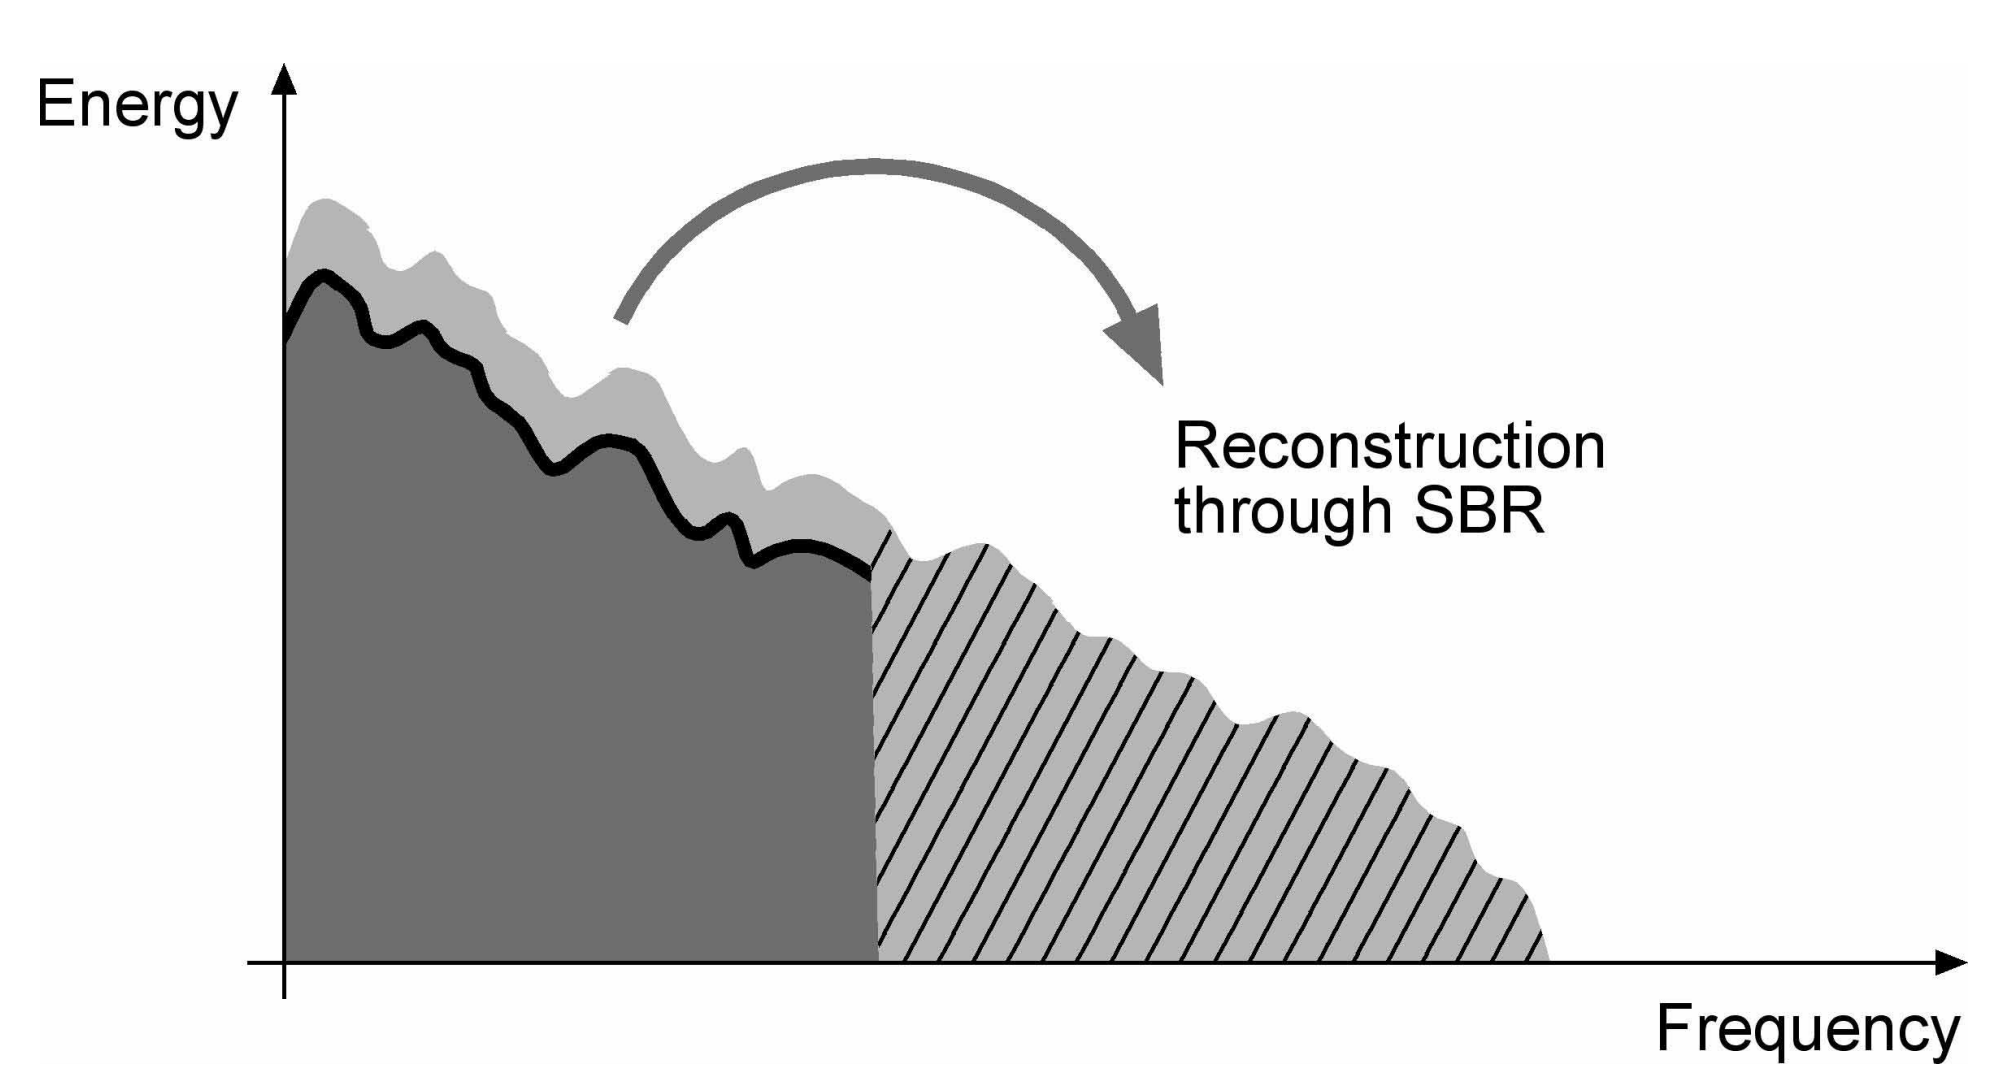
\includegraphics[width=.6\linewidth]{sbr}
\captionof{figure}{ \color{RoyalBlue} Principle of Bandwidth Extension (fig from \cite{dietz2002spectral}).}
\end{center}\vspace{1cm}

\begin{itemize}
  \item \textbf{Spectral band replication (SBR)$^*$}: M. Dietz, L. Liljeryd, K. Kjorling, and O. Kunz. "Spectral band replication, a novel approach in audio coding". In {\em Audio Engineering Society Convention}, 2002.
  \item \textbf{Non-negative matrix completion (NMC)}: D. Sun and R. Mazumder. Non-negative matrix completion for bandwidth extension: A convex optimization approach. In {\em 2013 IEEE International Workshop on Machine Learning for Signal Processing (MLSP)}, 2013.
  \item \textbf{Autoencoders$^*$}: M.~Miron and M.~E.~P. Davies. High frequency magnitude spectrogram reconstruction for music
    mixtures using convolutional autoencoders. In {\em In Proc. of the 21st Int. Conference on Digital Audio Effects
    (DAFx-18)}, 2018.
  \item \textbf{Sample based}: A. Gupta, B. Shillingford, Y. Assael, and T. Walters. Speech bandwidth extension with wavenet, 2019.
\end{itemize}
$^*$ will be considered as \textbf{baselines}.



\color{DarkSlateGray}

\section*{Model}
The architecture is a fully convolutional neural network with the following design :

\begin{minipage}[c]{.5\linewidth}
\begin{enumerate}
  \item $L$ layers followed by rectified linear units (ReLU) activations
  \item The number of output convolution channels $C$ is the same for all hidden layers
   \item Convolution kernels also share the same size $(K_t, K_f)$ in the time and frequency dimensions respectively
   \item padding by replicating their boundary values depending on the kernel size
   \item a fixed dilation ratio $D$ is used in the frequency dimension for hidden layers, and no dilation is used in the input and output layers of the network
\end{enumerate}
\end{minipage}
\begin{minipage}[c]{.5\linewidth}
  \hspace{2cm}\begin{center}\vspace{1cm}
  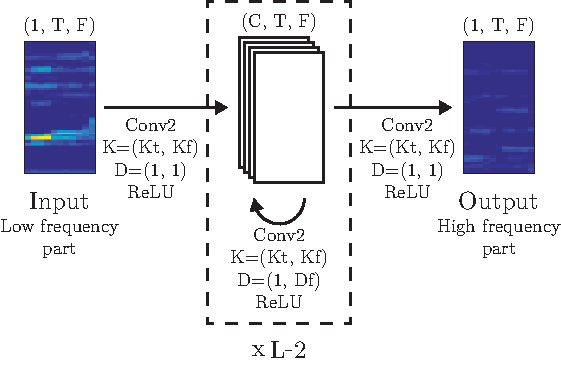
\includegraphics[width=.9\linewidth]{mdl}
  \captionof{figure}{ \color{RoyalBlue} Proposed deep convolutional neural network architecture for bandwidth extension.}
  \end{center}\vspace{1cm}
\end{minipage}

The model is trained using the mean squared error (MSE) loss function. Optimization is performed using the Adam algorithm with minibatches of $64$ examples and a learning rate of $0.001$.

\subsection*{A note on dilation}

\begin{minipage}[c]{.4\linewidth}
From a signal processing standpoint, this procedure is equivalent to applying the convolution on a down-sampled version of the input. As a result each hidden layer increases the receptive field by $D(K-1)$ frequency bins compared to $K-1$ without dilation.
\end{minipage}
\begin{minipage}[c]{.55\linewidth}
\begin{center}\vspace{1cm}
\includegraphics[width=.8\linewidth]{dilation2}
\captionof{figure}{ \color{RoyalBlue} Dilation can be viewed as a convolution on a downsampled version of the input (fig from \cite{tan2018gated}).}
\end{center}\vspace{1cm}
\end{minipage}

\section*{Experiments}

\begin{center}\vspace{1cm}
\begin{tabular}{cc}
  (a) & (b) \\
  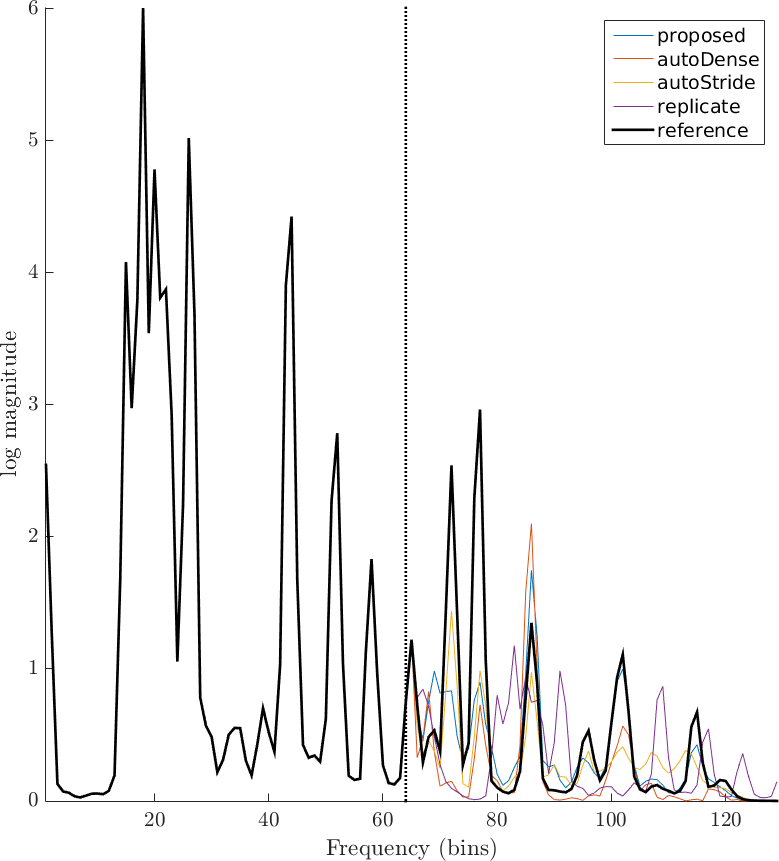
\includegraphics[width = .45\columnwidth]{solos_1141.png}
&
  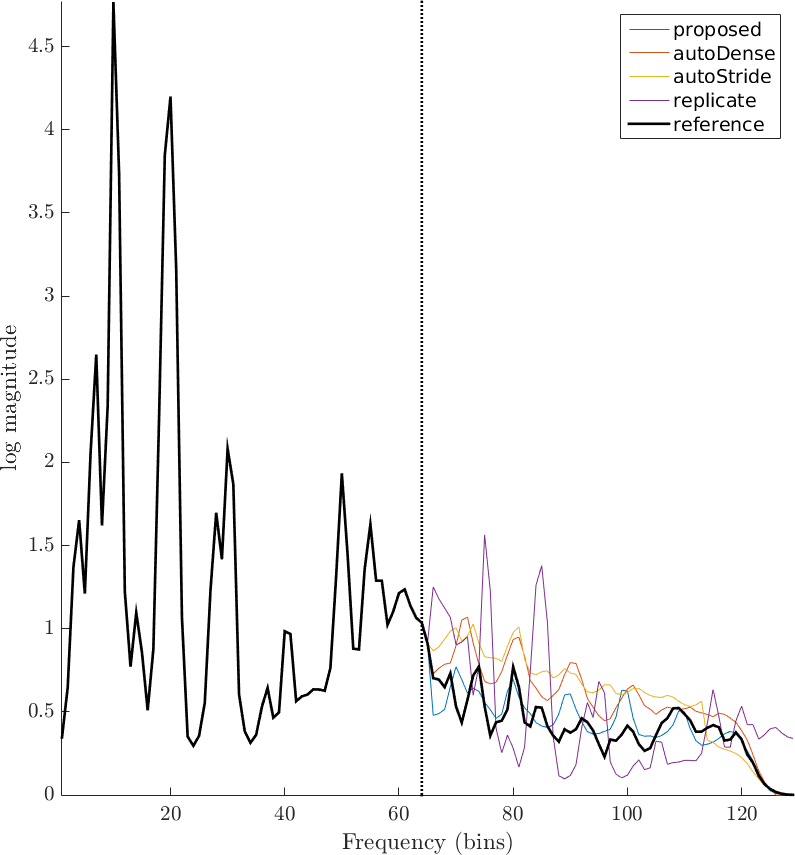
\includegraphics[width = .45\columnwidth]{gtzan_1120.png}
\end{tabular}
\captionof{figure}{ \color{RoyalBlue} Examples of predictions for (a) the \textit{medley-solos-db} dataset and (b) the \textit{gtzan} dataset. The proposed model handles correctly the harmonic structures (a) and the average magnitude of more complex spectral shapes (b).}
\end{center}\vspace{1cm}

\begin{minipage}[c]{.55\linewidth}
  \begin{center}
\begin{tabular}{lcc|cc}
  & \multicolumn{2}{c|}{\textit{medley-solos-db}} & \multicolumn{2}{c}{\textit{gtzan}} \\
  method & mirror & oracle & mirror & oracle \\
\hline
null & \textbf{12.9 $\pm$3} & 12.9 $\pm$3 & \textbf{12.9 $\pm$3} &  12.9 $\pm$3\\
replicate & 10.7 $\pm$3 & 11.6 $\pm$3 & 10.8 $\pm$3 & 13.3 $\pm$3\\
\hline
cnn bottleneck & 10.6 $\pm$2 &  13.3 $\pm$3 & 11.1 $\pm$3 & 15.6 $\pm$3 \\
cnn stride2 & 11.2 $\pm$3 & 13.9 $\pm$3 & 11.2 $\pm$3 & 15.6 $\pm$3 \\
\hline
proposed  & 11.0 $\pm$2 & 14.3 $\pm$3  & 11.3 $\pm$3 & 16.3 $\pm$3 \\
\hline
oracle & 10.5 $\pm$3 & $\infty$ & 10.5 $\pm$3 & $\infty$ \\
\end{tabular}
\captionof{figure}{ \color{RoyalBlue} SRR achieved by the different methods on the \textit{medley-solosdb} and the \textit{gtzan} datasets using the \textit{mirror} and \textit{oracle} phase estimates.}
\end{center}
\end{minipage}
\begin{minipage}[c]{.4\linewidth}
\begin{center}
\begin{tabular}{lcc}
method & \textit{medley-solos-db} & \textit{gtzan} \\
\hline
null & 15.4$\pm$2.9 & 13.0$\pm$1.9  \\
replicate & 25.6$\pm$3.6 & 29.7$\pm$4.9 \\
\hline
cnn bottleneck & 31.7 $\pm$3.2 & 40.6 $\pm$5.8 \\
cnn stride2 & 33.3 $\pm$2.7 & 36.9 $\pm$ 5.7 \\
\hline
proposed & \textbf{34.2 $\pm$3.2} & \textbf{42.9 $\pm$5.7} \\
\hline
oracle  & 75.2$\pm$9.3 & 78.4$\pm$10.9  \\
\end{tabular}
\captionof{figure}{ \color{RoyalBlue} OPS using the mirror phase estimate.}
\end{center}
\end{minipage}


\section*{Experimental protocol}
\label{sec:protocol}

\subsection*{Datasets}

\begin{enumerate}
  \item \textit{medley-solos-db}: 18 hours, monophonic
  \item \textit{gtzan}: 8 hours, polyphonic
\end{enumerate}

\subsection*{Pre-processing}

\begin{enumerate}
  \item resampling to $8$kHz
  \item short-term Fourier transform with frame size of $256$ samples, hop size of $128$ samples and a Hann window.
  \item "textures" of $10$ frames, processed as individual examples.
\end{enumerate}

\subsection*{Metrics}

Three metrics are considered:
\begin{enumerate}
  \item \textbf{Spectral loss} : the loss used to optimize the network
  \item \textbf{SRR} : signal to reconstruction ratio computed in the time domain
  \item \textbf{OPS} : overall perceptual score from the PEASS toolkit \cite{emiya2011subjective}
\end{enumerate}

\subsection*{Anchors and baselines}

Two anchors are considered:
\begin{enumerate}
  \item \textit{oracle}: the predicted magnitude in the high frequencies are the actual ones
  \item \textit{null}: the predicted magnitude in the high frequencies are set to zero
\end{enumerate}

Three baselines are considered:
\begin{enumerate}
  \item \textit{sbr}: crude implementation of the SBR technique
  \item \textit{cnn bottleneck}: reimplementation of architecture proposed in \cite{miron2018high}
  \item \textit{cnn stride2}: reimplementation of architecture proposed in \cite{miron2018high}
\end{enumerate}

\color{SaddleBrown} % SaddleBrown color for the conclusions to make them stand out

\section*{Forthcoming Research}

\begin{enumerate}
  \item \textbf{advanced phase estimators}
  \item \textbf{mismatch between training and testing audio material}
  \item \textbf{creative use} : predicting the high frequency spectra of a 'pop' song using network trained on 'country' songs may be of creative interest, to explore the yet to be defined notion of \textbf{musical style transfer}.
\end{enumerate}


\color{DarkSlateGray}

\section*{Acknowledgements}


The authors would like to acknowledge partial support from ANR project Cense (grant ANR-16-CE22-0012).

\bibliographystyle{../paper/IEEEbib} % Plain referencing style
\bibliography{bib}

%----------------------------------------------------------------------------------------

\end{multicols}
\end{document}
